\documentclass[10.5pt,onecolumn,a4paper]{article}%pre,aps,
\usepackage{ctex}
\usepackage{setspace,dcolumn}
\usepackage{graphicx}
\usepackage{float,psfrag,epsfig}
\usepackage{hyperref}
%\usepackage[font=small,format=plain,labelfont=bf,textfont=it,justification=raggedright,singlelinecheck=false]{caption}
\usepackage{enumerate}
\usepackage{amsmath}
\usepackage{longtable,tabularx,multirow}
\hypersetup{colorlinks=true}
\usepackage{geometry}
\geometry{top=2.54cm,bottom=2.54cm,left=3cm,right=3cm}
\usepackage{subcaption}
\usepackage{caption}
\usepackage{booktabs}%excel2latex
\usepackage{multirow}
\usepackage{multicol}
\usepackage{colortbl}%表格背景色
\usepackage{listings,xcolor}
\usepackage{array}
\usepackage{framed}
\lstset{frame=shadowbox,rulesepcolor=\color{red!20!green!20!blue!20}, %边框阴影
        numbers=left, %设置行号位置
        numberstyle=\tiny, %设置行号大小
        basicstyle=\tiny, %代码字体大小设定
        keywordstyle=\color{blue}, %设置关键字颜色
        commentstyle=\color[cmyk]{1,0,1,0}, %设置注释颜色
        %frame=single, %设置边框格式
        escapeinside=``, %逃逸字符(1左面的键),用于显示中文
        breaklines, %自动折行
        extendedchars=false, %解决代码跨页时,章节标题,页眉等汉字不显示的问题
        xleftmargin=2em,xrightmargin=2em, aboveskip=1em, %设置边距
        tabsize=4, %设置tab空格数
        showspaces=false %不显示空格
       }
   
\makeatletter
\def\verbatim{\scriptsize\@verbatim \frenchspacing\@vobeyspaces \@xverbatim}
\makeatother
   
   

\title{美国FOF市场总资产的时间序列分析}
\author{祁周, 王喆, 任庆杰}

\begin{document}

\begin{titlepage}	
	\begin{center}	
		
\includegraphics[width=0.2\textwidth]{./pkulogo}\\[1cm]    
		
		\textsc{\LARGE Peking University}\\[1.5cm]
		
		\textsc{\Large }\\[2cm]
		
		
		% Title

		{ \huge \bfseries FOF基金时间序列分析}\\[3cm]

		
		% Author and supervisor
		\begin{minipage}{0.4\textwidth}
			\begin{flushleft} \large
				\emph{\Large 作者:}\\
				\Large 祁周\\
				\Large 王喆\\
				\Large 任庆杰
			\end{flushleft}
		\end{minipage}
		\begin{minipage}{0.4\textwidth}
			\begin{flushright} \large
				\emph{\Large 指导老师:} \\
		\Large 涂云东
			\end{flushright}
		\end{minipage}
		
		\vfill
		
		% Bottom of the page
		{\large \today}
		
	\end{center}
	
\end{titlepage}






\begin{abstract}

\end{abstract}
\clearpage

\section{引言}
基金中基金(fund of funds,简称FOF)是指投资于其他基金组合的基金.在欧美市场,基金中基金已经发展成为数量和规模均较大的一类成熟的理财产品.在美国市场上, FOF市场总资产在1995年初仅有3891.54百万美元,到2016年底已发展为1439637.04百万美元,年均增长率高达30.84\%.

2016年9月,中国证券监督管理委员会发布《公开募集证券投资基金运作指引第2号------基金中基金指引》,标志着公募基金行业迎来创新品种FOF,并由此进入FOF发展的全新时代.
\subsection{基金中基金的起源}

基金中基金起源于上世纪70年代,最初是以其他私募股权基金(private equity fund)为投资的标的.这是因为私募股权基金往往设置有非常高的投资门槛,单笔投资的资金规模巨大,并且要求参与者为合格投资者,这使得许多有意愿投资私募股权基金的个人投资者被拒之门外.而PE FOF作为渠道,解决了这个问题,使得个人投资者可以通过投资PE FOF,即间接地投资一篮子私募股权基金,来分享风险投资可能带来的高收益.

与中国市场不同,美国法律对于没有明确规定禁止的事情,默认为许可,而在中国,公民仅能做法律允许的事.这使得美国资本市场的创新能力非常强大,非常有利于全新产品的创立.

\subsection{基金中基金的成熟契机}

1987年10月19日,美国股票市场在经历了两年的牛市之后,遭受到一次巨大的股灾,这也是历史上继1929年经济危机后第二次全球经济危机.道琼斯指数单日跌幅达22\%,恒生指数暴跌11\%,这促使投资者开始思考如何根据市场的不同情况配置不同种类的基金,分散标的,减小风险.

\begin{figure}[ht]
\begin{minipage}[ht]{0.47\textwidth}
\centering
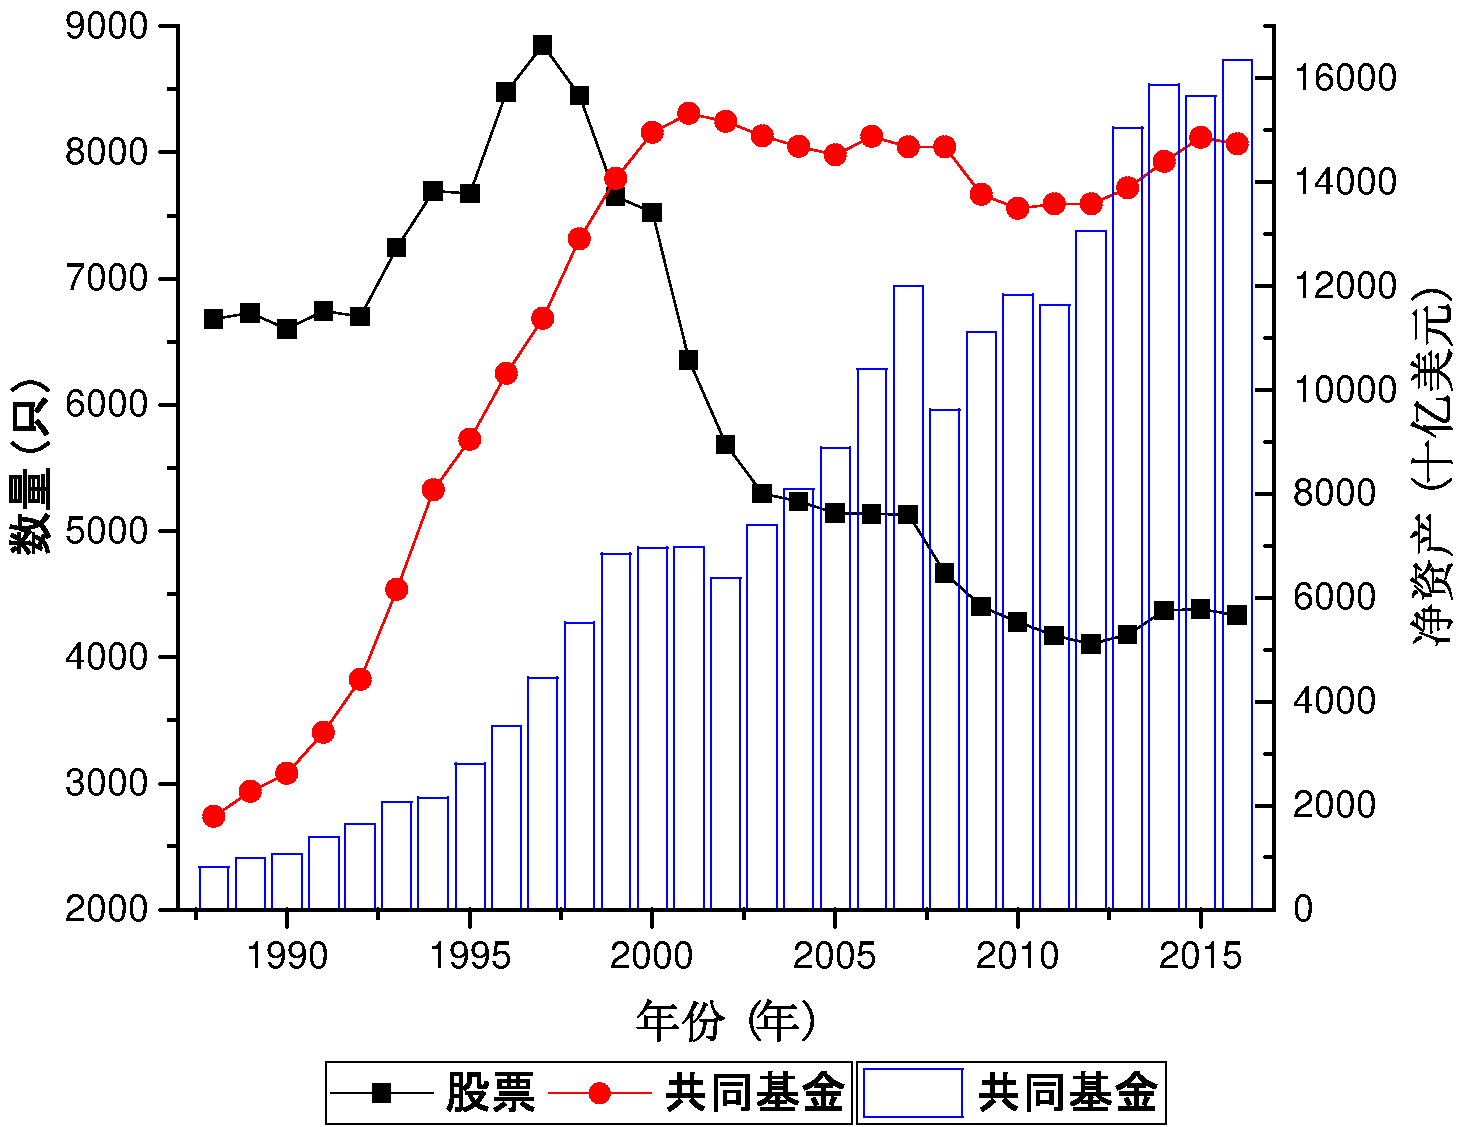
\includegraphics[width=\textwidth]{pic/mutual.pdf}
\subcaption{}\label{fg:mutual}
\end{minipage}%
\hspace{0.06\textwidth}
\begin{minipage}[ht]{0.47\textwidth}
\centering
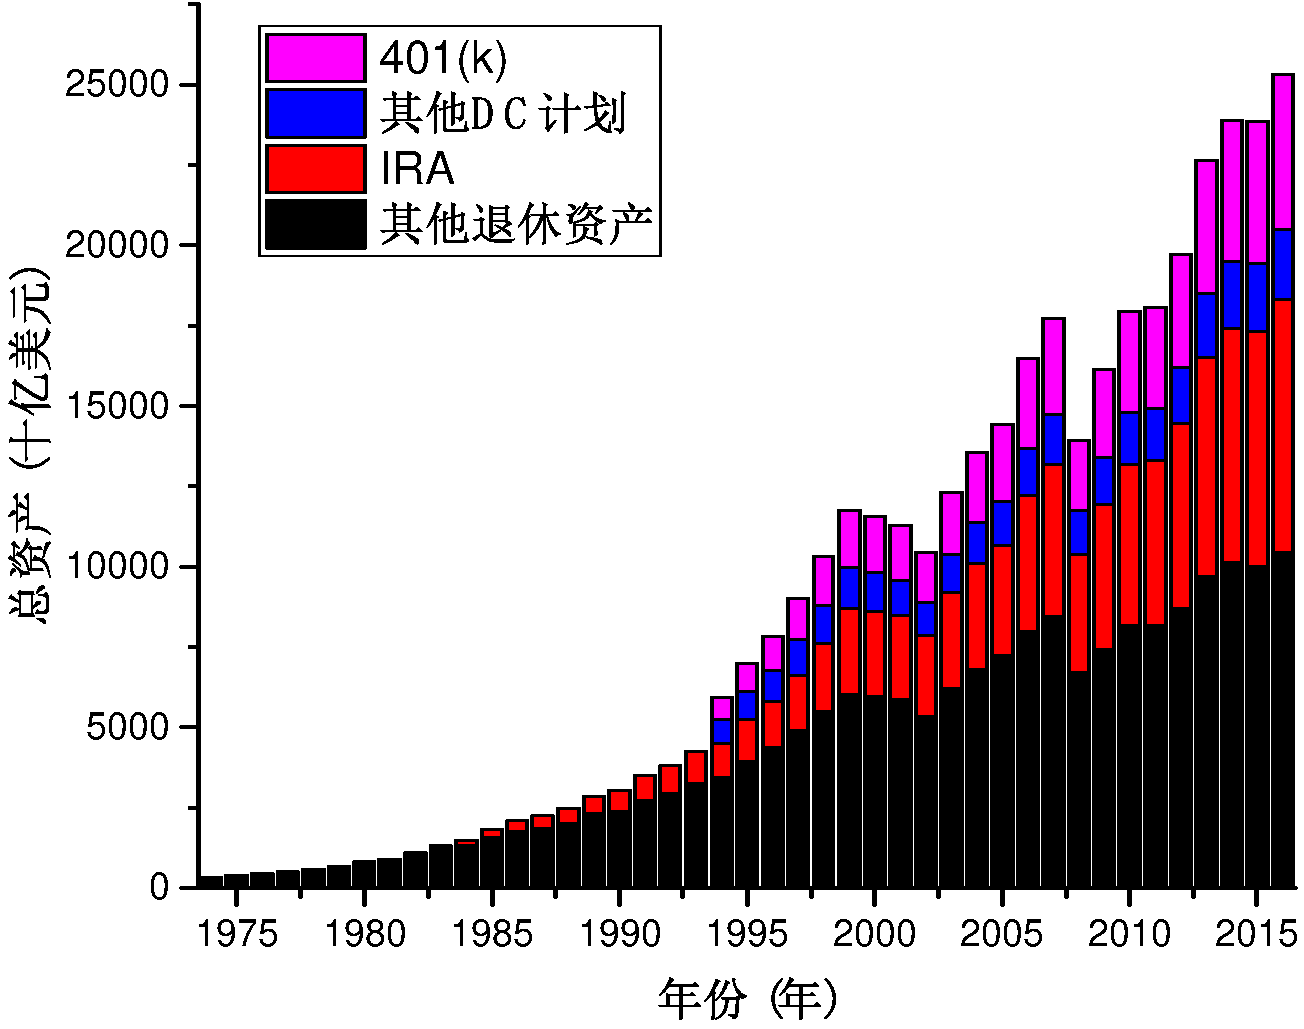
\includegraphics[width=\textwidth]{pic/retirement.pdf}
\subcaption{}\label{fg:retirement}
\end{minipage}
\caption{美国FOF基金相关市场发展:(a)1988--2016年美国股票、共同基金市场发展状况;(b)1974--2016年美国退休养老资产发展状况}
\end{figure}

共同基金在这次惨重的股灾过后,也不断开发出新的产品,基金的类型迅速增多,整个基金市场呈现爆发式增长,如图~\ref{fg:mutual}~所示,基金数量甚至远超股票数量.市场的复杂性、基金的多样性使得投资者对基金筛选及风险分散有了极大的需求,从此, FOF市场规模的扩大有了客观上的推动因素.

在同一时期,美国也大规模推广401(k)计划,这个计划的主要内容是创建了一个税收优惠账户,对雇员和雇主共同缴纳的养老金进行投资过程中收取的股息税和资本利得税进行减免.这为随后养老金进入资本市场打开了通道.

\subsection{基金中基金与养老金的关系\label{sec:retire}}

如上文所述,退休养老资产的扩大成为了美国基金中基金市场规模扩大的重要因素.为了能够吸引养老金投资者,基金公司推出了大量的针对养老金需求的基金中基金产品. 尽管FOF具有双重收费的劣势, 但它双重风险分散、多样化投资的优势吸引了大量养老金投资者的青睐.

在养老资产的构成中, DB(Defined Benefit) Plan 和年金(Annuity)都是由雇主或政府进行统一管理, 而 IRA 计划和 DC(Defined Contribute) Plan 则由雇员定期缴纳后进行投资. 由于养老金账户是自动从薪水中扣除, 所以养老金资产的序列会更加平稳, 时间相依性更弱. 退休养老基金主要投资于基金中基金产品,而基金中基金市场的主要资金来源也是退休养老基金,二者相互依存.基金中基金解决了养老金投资的难点,将两者紧密联系在一起.

\subsection{美国FOF市场的总资产序列}
根据彭博资讯提供的数据可以获取美国市场上所有FOF基金的规模及成立时间,以此统计出全市场的数量和规模,如图~\ref{fg:fof}~所示,时间区间为1995年1月至2017年5月,具体数据如表~\ref{tab:fof}~所示.
\begin{figure}[ht]
  \centering
  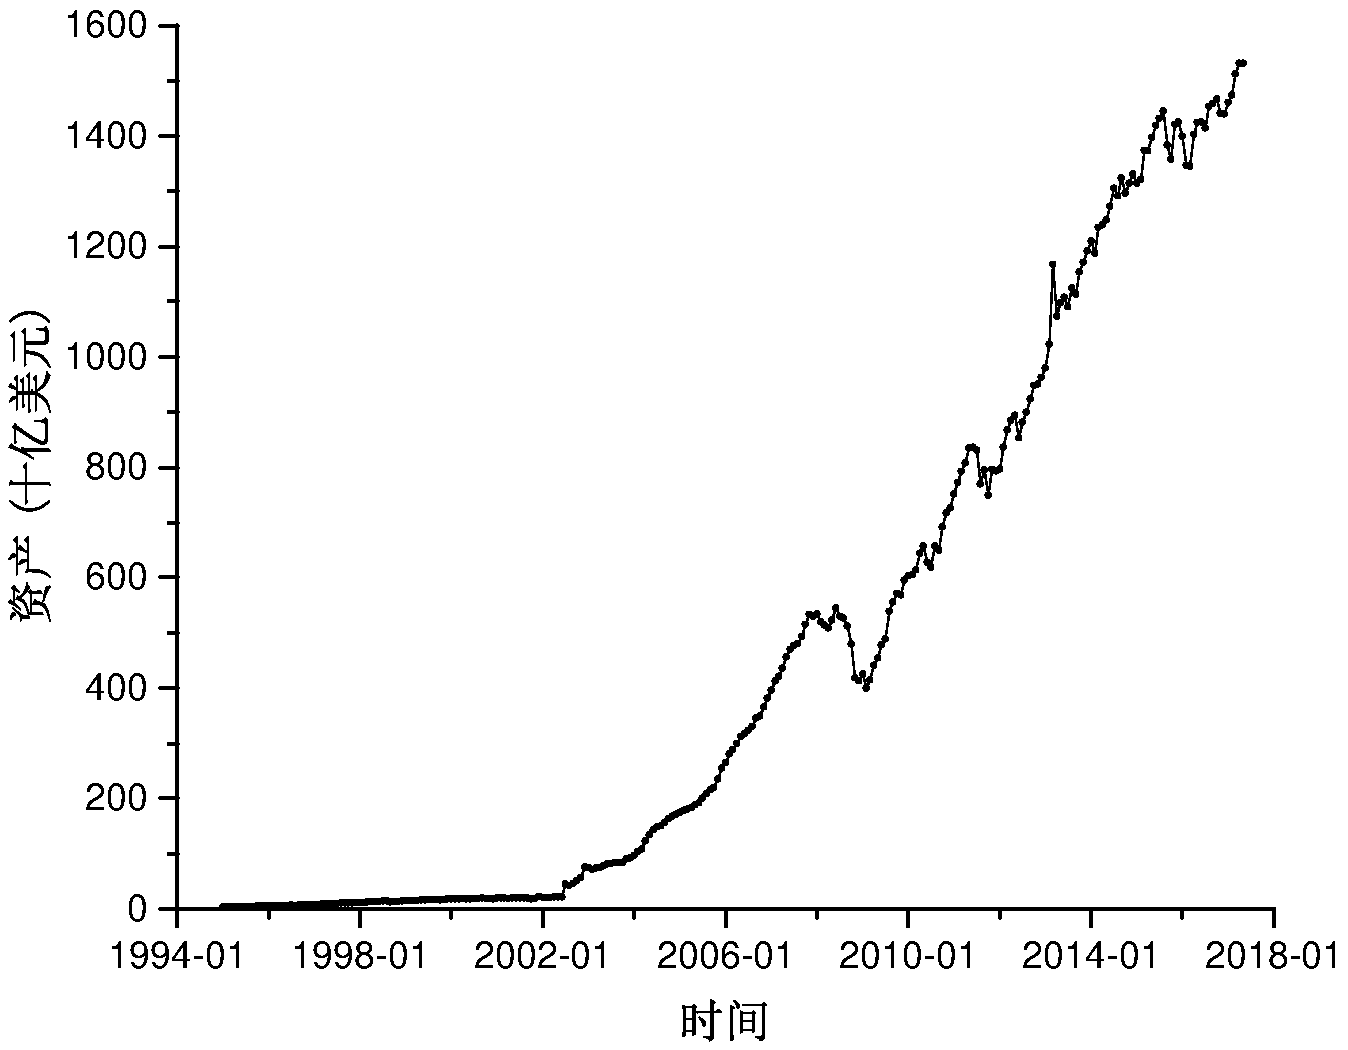
\includegraphics[width=0.6\textwidth]{pic/fof.pdf}
  \caption{1995年以来美国基金中基金市场的规模}\label{fg:fof}
\end{figure}

如图~\ref{fg:fof}~所示,美国基金中基金市场的资产规模呈上升趋势,显示出明显的时间趋势.



\section{美国FOF市场总资产建模}

\subsection{对资产对数增长率建立MA(5)模型}
首先利用ADF检验美国FOF总资产序列是否存在单位根, 在备择假设为平稳性的条件下, 对FOF基金的资产总量序列$\{ast\}$进行检验. 检验结果为$P=0.8158$, 这说明FOF的资产总量数据并不是一个平稳的时间序列. 而对FOF资产总量取对数差分后,即得到总资产的对数增长率序列$\{GR\_ast\}$,如图\ref{fig:unnamed-chunk-1-2}所示


\begin{figure}[h!]
	\centering
	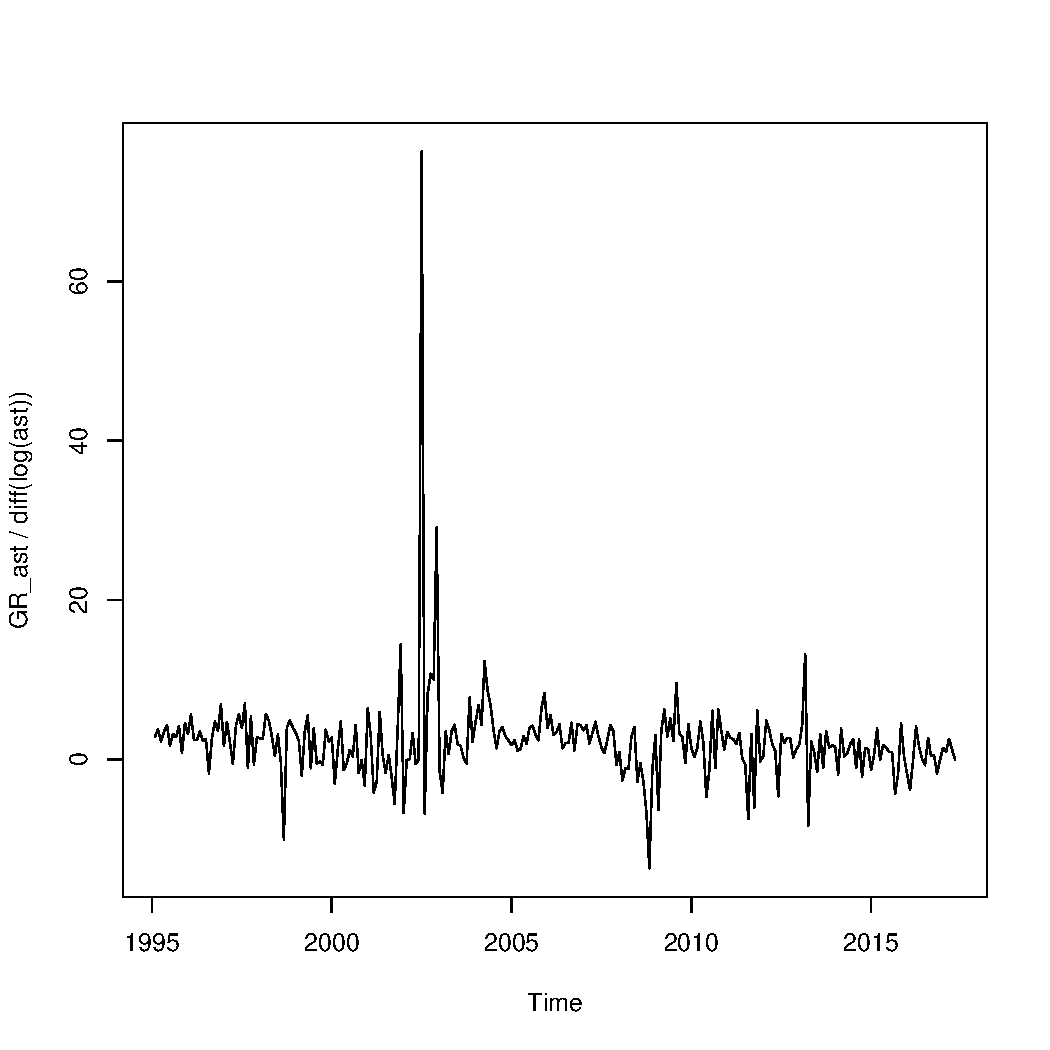
\includegraphics[width=0.6\linewidth]{pic/ast/unnamed-chunk-1-2}
	\caption{美国FOF基金总资产的对数增长率序列}
	\label{fig:unnamed-chunk-1-2}
\end{figure}
 再次进行ADF检验, 检验结果$P<0.01$, 拒绝了非平稳的原假设, 即其对数差分后是一个平稳序列.具体的R语言结果如下所示:
\begin{framed}
		 \begin{verbatim}
		 Augmented Dickey-Fuller Test
		 data:  ast
		 Dickey-Fuller = -1.4307, Lag order = 6, p-value = 0.8158
		 alternative hypothesis: stationary
		\end{verbatim}
	\end{framed}
\begin{framed}
	\begin{verbatim}
 	Augmented Dickey-Fuller Test 
   data:  GR_ast
   Dickey-Fuller = -4.9254, Lag order = 6, p-value = 0.01
   alternative hypothesis: stationary
	\end{verbatim}
\end{framed}
对对数差分后的序列进行ARMA建模. 见图\ref{gr_ast_ape}, 此序列的ACF函数在5阶处截尾, PACF函数在5阶处结尾,EACF显示应为MA(5) .
\begin{figure}[h!]
	\begin{minipage}[ht]{0.3\textwidth}
		\centering
		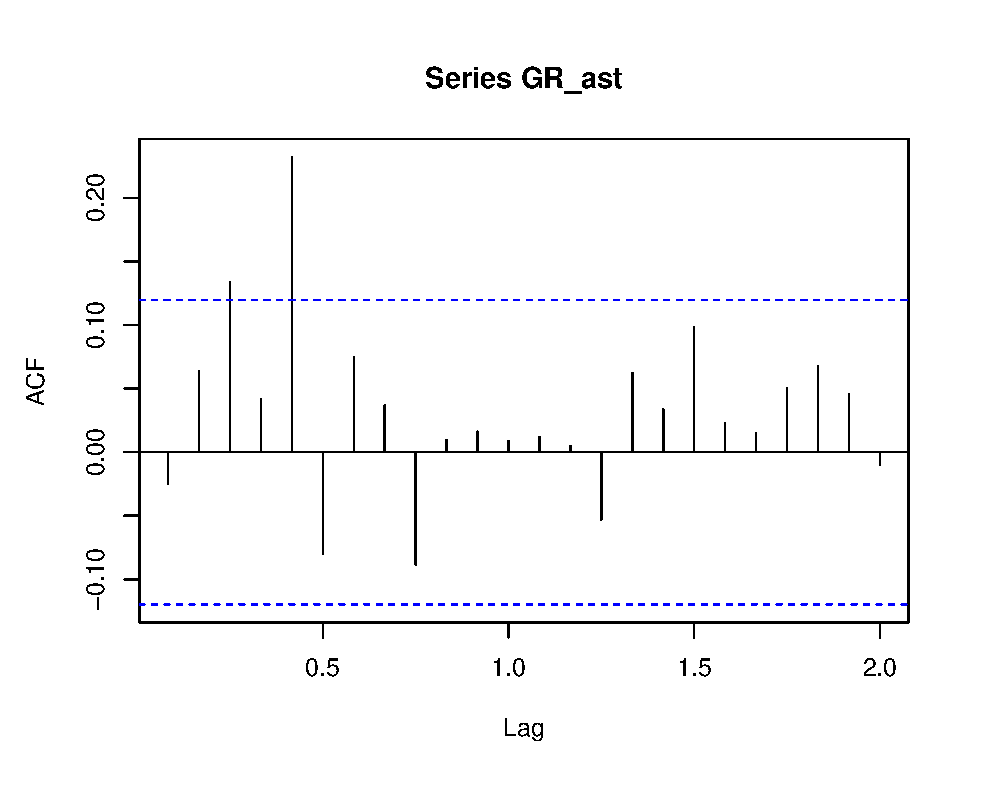
\includegraphics[width=\textwidth]{pic/ast/acf(gr_ast)}
		\subcaption{}\label{acf(gr_ast)}
	\end{minipage}%
	\hspace{0.04\textwidth}
	\begin{minipage}[ht]{0.3\textwidth}
		\centering
		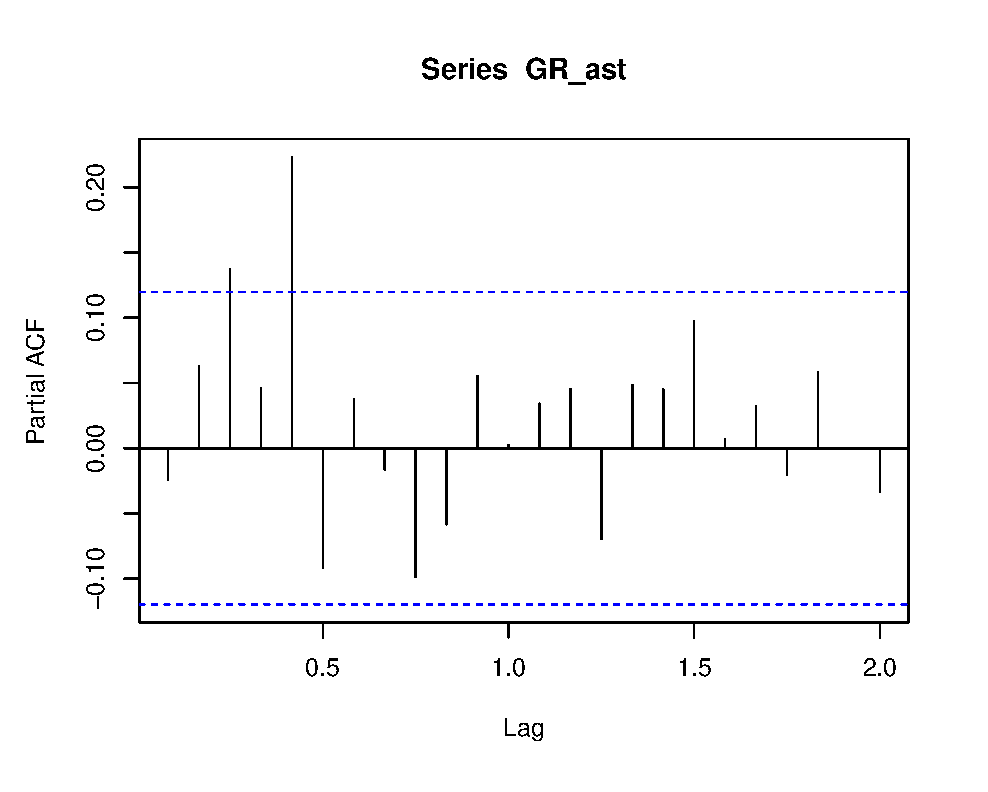
\includegraphics[width=\textwidth]{pic/ast/pacf(gr_ast)}
		\subcaption{}\label{pacf(gr_ast)}
	\end{minipage}
	\hspace{0.04\textwidth}
	\begin{minipage}[ht]{0.3\textwidth}
	\centering
	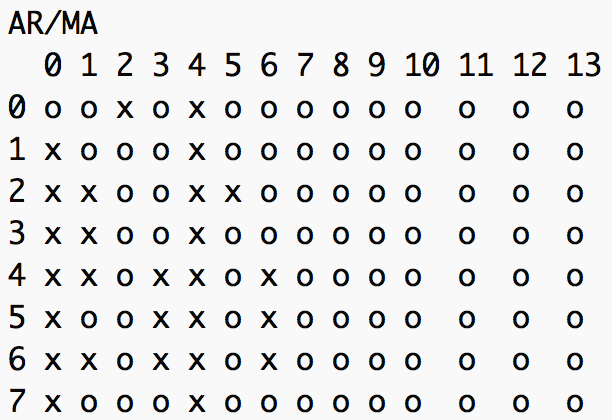
\includegraphics[width=1\textwidth]{pic/ast/eacf(gr_ast)}
	\subcaption{}\label{eacf(gr_ast)}
\end{minipage}
	\caption{GR\_ast序列的相关性: (a):ACF of GR\_ast; (b):PACF of GR\_ast; (c):EACF of GR\_ast}\label{gr_ast_ape}
\end{figure}
\emph{经过反复尝试,} 当使用MA(5)对序列进行刻画时, 可以得到较好的估计效果,且ma1,ma2和ma4都不显著,置0. MA(5)模型的极大似然估计结果如下:
\begin{framed}
\begin{verbatim}
 Call:
 arima(x = GR_ast, order = c(0, 0, 5), fixed = c(0, 0, NA, 0, NA, NA))
 Coefficients:
       ma1  ma2     ma3  ma4     ma5  intercept
         0    0  0.1352    0  0.2156     2.2333
 s.e.    0    0  0.0616    0  0.0556     0.4705
 sigma^2 estimated as 32.79:  log likelihood = -848.09,  aic = 1702.18
\end{verbatim}
\end{framed}





\subsection{模型诊断与异常值处理}

对上述模型的残差序列$r$进行Ljung-Box检验,如下:
\begin{framed}
\begin{verbatim} 
 	 	Box-Ljung test	 
 	 data:  r
 	 X-squared = 15.522, df = 22, p-value = 0.8389
\end{verbatim}
\end{framed}
$p-value=0.8389$ ,满足白噪声要求,说明$r$序列不存在一阶自相关.继续对残差$r$序列进行 McLeod.Li检验,见图\ref{mcr} ,检验结果各阶的$P$值都接近1, 说明不存在ARCH效应.具体的结果如图\ref{testr}所示,可以看到残差序列及残差平方序列的自相关性都很小,可以认为无自相关性。
\begin{figure}[h!]
	\begin{minipage}[ht]{0.31\textwidth}
		\centering
		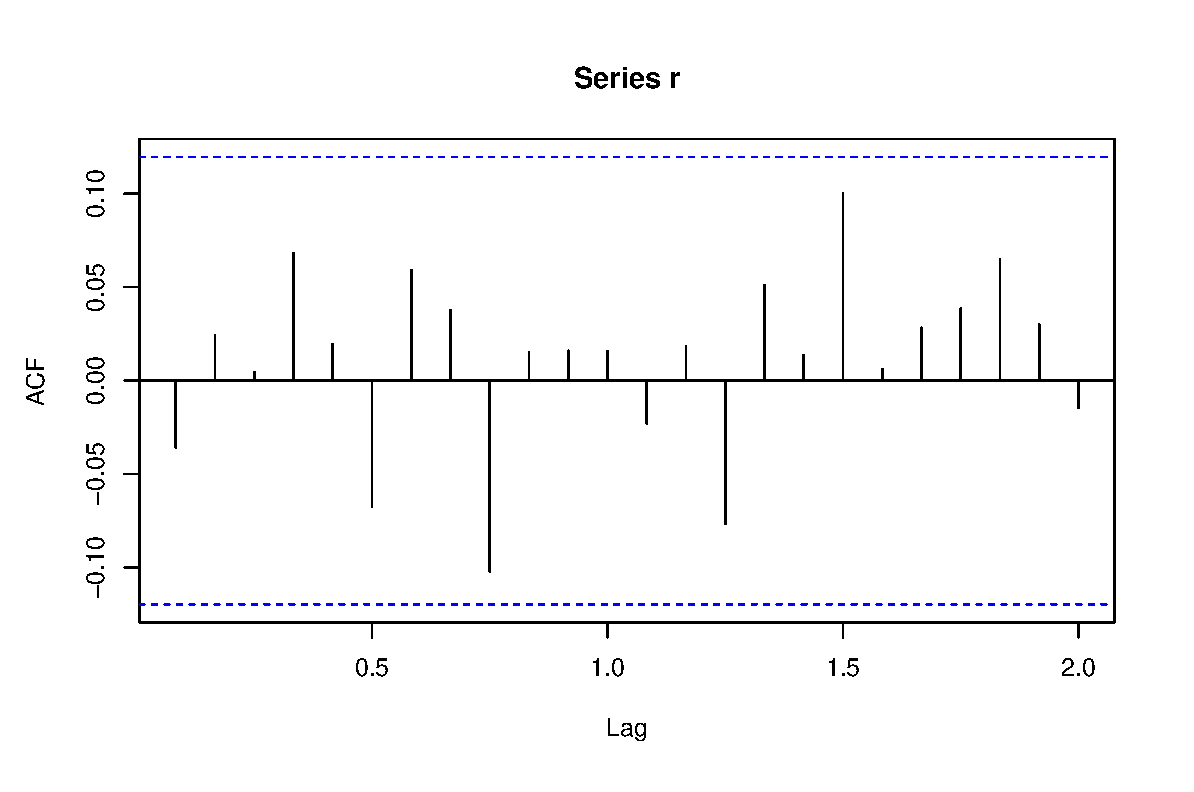
\includegraphics[width=\textwidth]{pic/ast/acfr}
		\subcaption{}\label{acfr}
	\end{minipage}%
	\hspace{0.02\textwidth}
	\begin{minipage}[ht]{0.31\textwidth}
		\centering
		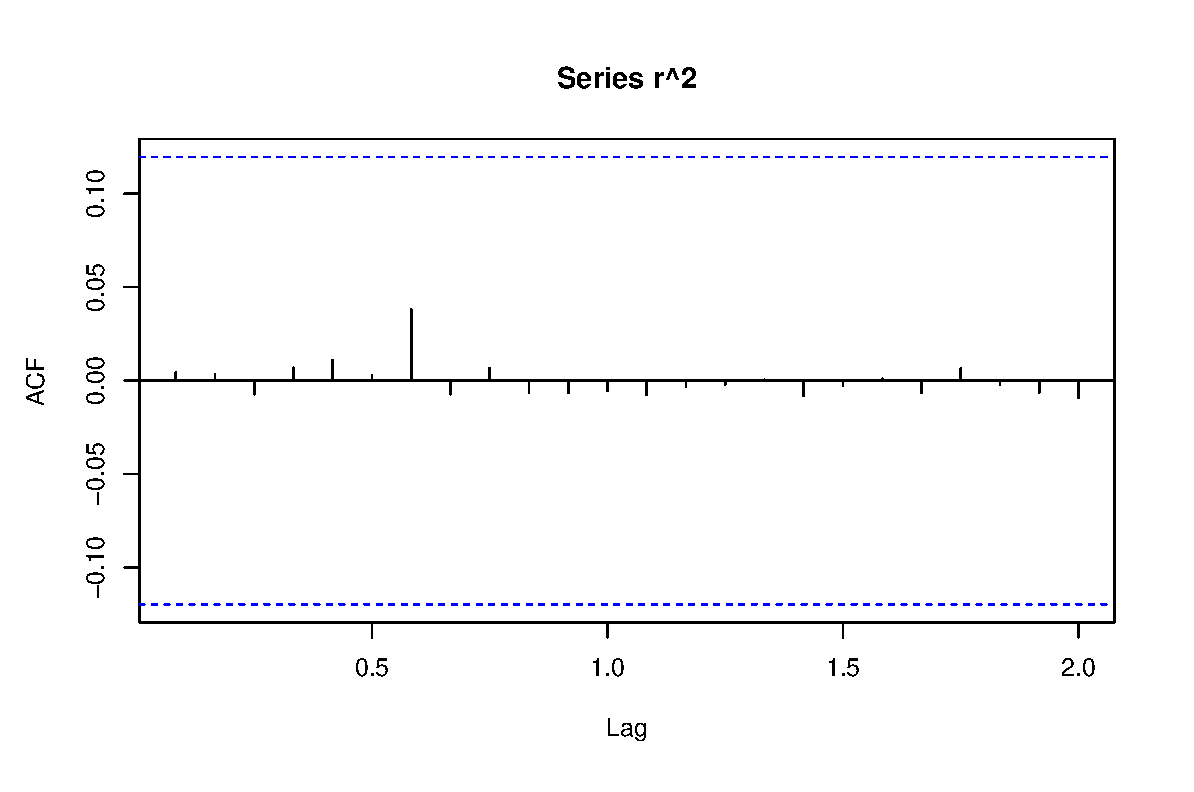
\includegraphics[width=\textwidth]{pic/ast/acfr2}
		\subcaption{}\label{acfr2}
	\end{minipage}
	\hspace{0.02\textwidth}
	\begin{minipage}[ht]{0.31\textwidth}
		\centering
		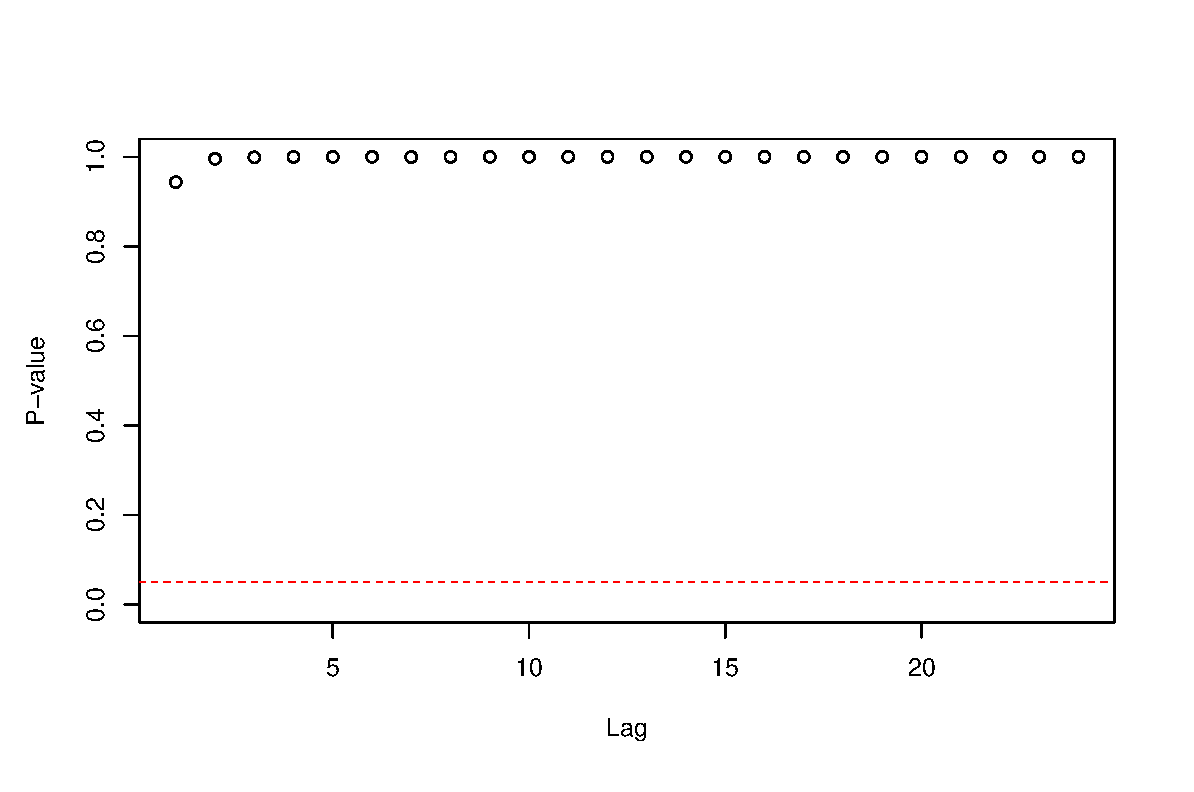
\includegraphics[width=1\textwidth]{pic/ast/mcr}
		\subcaption{}\label{mcr}
	\end{minipage}
	\caption{GR\_ast序列的MA(5)模型的残差序列相关性: (a):ACF of r; (b):ACF of r$^2$; (c):McLeod.Li.test of r}\label{testr}
\end{figure}

但进一步绘制出标准化的残差图, 见图\ref{fig:srgrast}
\begin{figure}
	\centering
	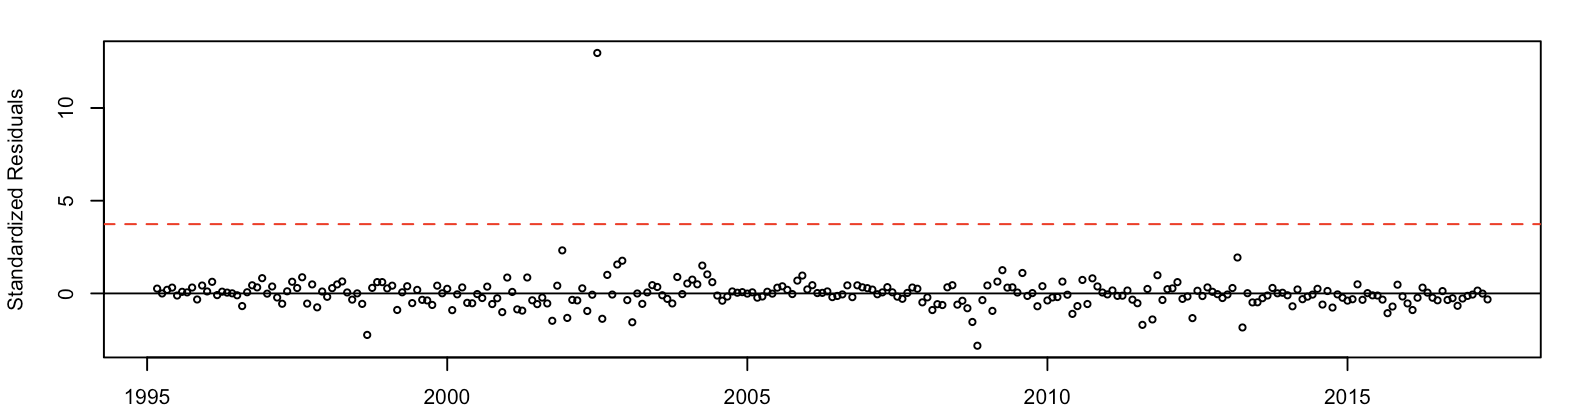
\includegraphics[width=0.8\linewidth]{pic/ast/srgr_ast}
	\caption{GR\_ast序列的MA(5) 模型的标准化残差}
	\label{fig:srgrast}
\end{figure}
发现在第90期有一个明显的异常值. 因为这个异常值的出现, 使得其他残差的尺度都会被缩小,很可能使得在模型诊断时,其他残差出现的波动聚类现象被忽略. 我们利用R语言中的detectIO()与detectAO()\footnote{其中IO和AO分别为新息异常值和可加异常值,具体原理的利用了 Chang, Chen and Tia在1998年提出的$\lambda_{1,T}$和$\lambda_{2,T}$统计量。}函数进行模型检测,也得到第90期为异常值的结果,且为IO异常值。为了削弱第90期的异常值对模型的影响, 令
\begin{equation}
GR\_ast[90] = \frac{1}{3} \cdot (GR\_ast[89]+GR\_ast[90]+GR\_ast[91])
\end{equation}
如图\ref{ioad}分别为原序列与进行异常值处理后的序列,从图\ref{ad}可看出波动有聚类现象。
\begin{figure}[h!]
	\begin{minipage}[ht]{0.48\textwidth}
		\centering
		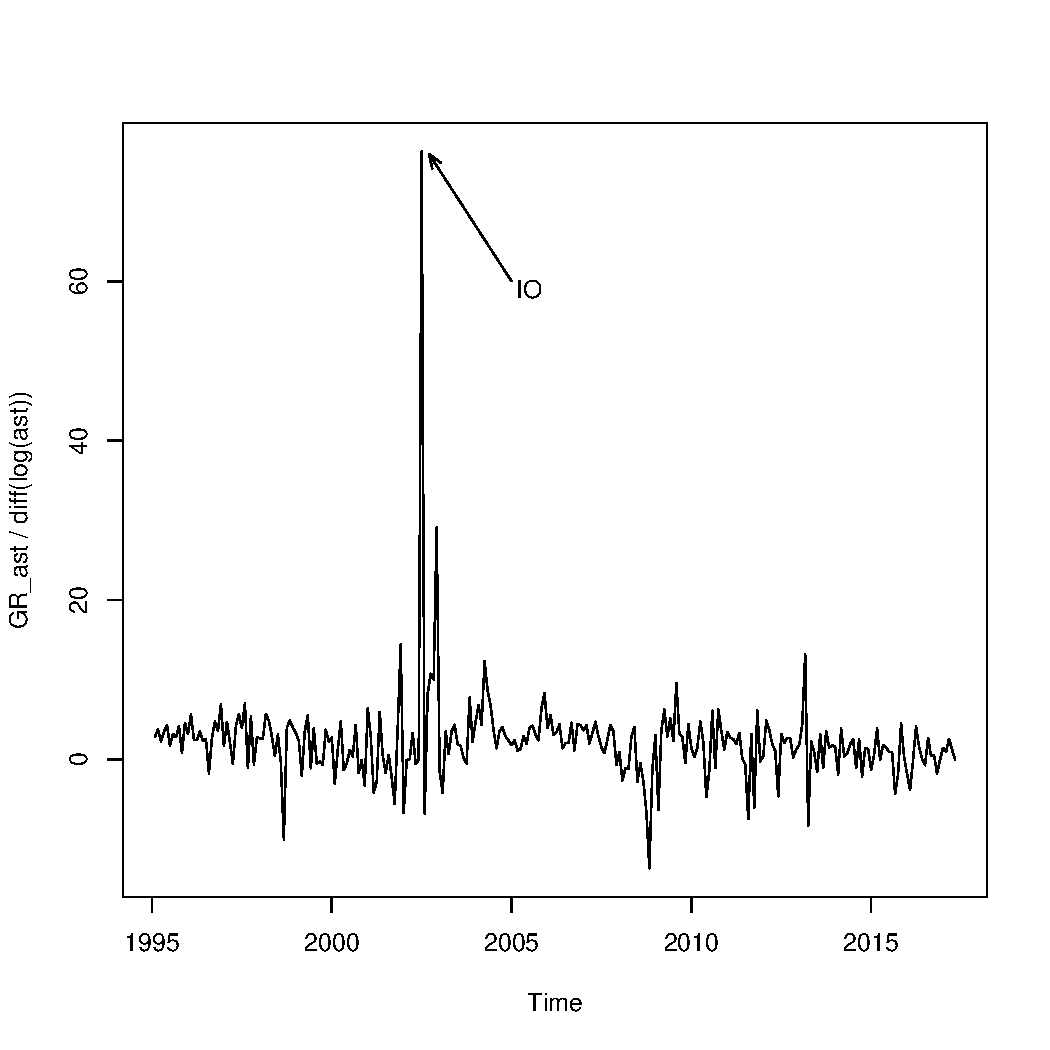
\includegraphics[width=0.7\textwidth]{pic/ast/unnamed-chunk-1-6}
		\subcaption{}\label{io}
	\end{minipage}%
	\hspace{0.04\textwidth}
	\begin{minipage}[ht]{0.48\textwidth}
		\centering
		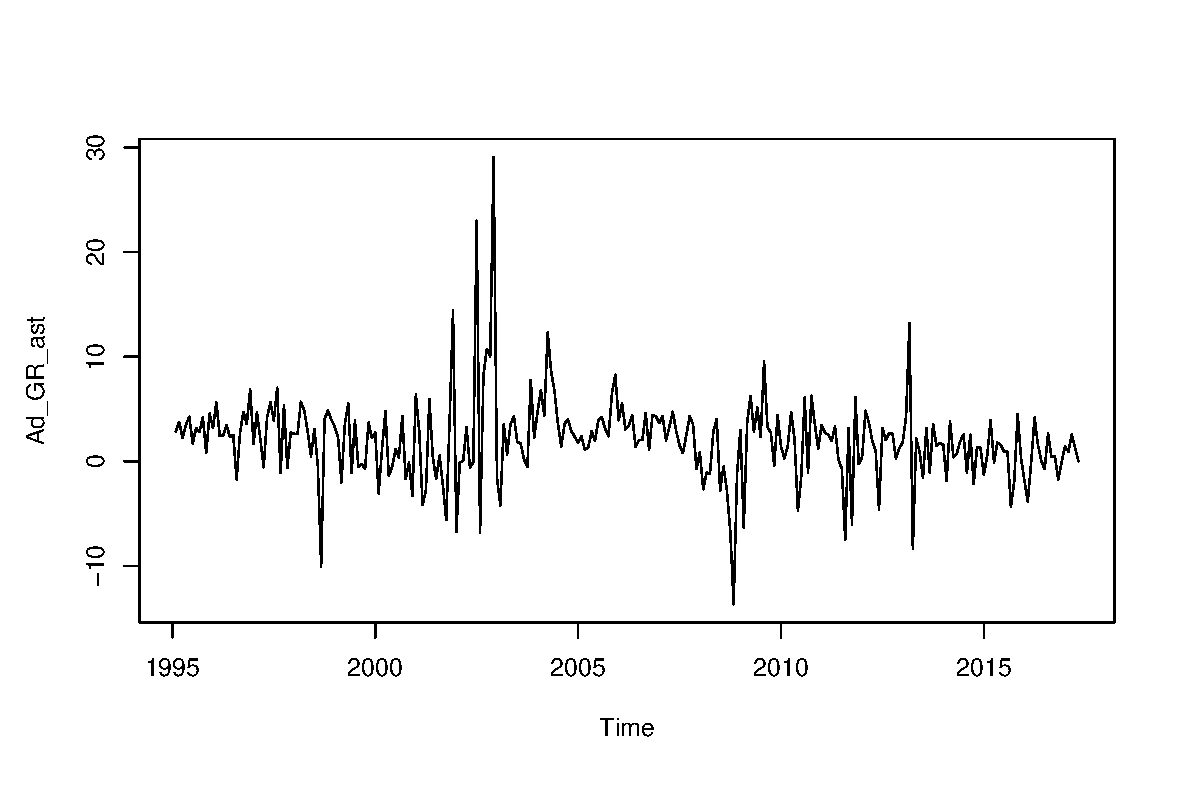
\includegraphics[width=\textwidth]{pic/ast/adgrast}
		\subcaption{}\label{ad}
	\end{minipage}
	\caption{进行异常值处理前后的GR\_ast序列: (a):未处理的GR\_ast序列; (b):进行异常值处理后的GR\_ast序列}\label{ioad}
\end{figure}






\subsection{对调整后的序列建立ARMA(0,5)-GARCH(1,1)模型}
序列进行异常值调整后,首先对其建立ARMA模型,与前面建立MA模型的方法一样,利用序列的ACF、PACF与EACF定阶,然后依旧建立了一个MA(5)模型,其参数的具体估计结果如下
\begin{framed}
\begin{verbatim} 
 Call:
 arima(x = Ad_GR_ast, order = c(0, 0, 5), fixed = c(0, 0, NA, 0, NA, NA))
 Coefficients:
       ma1  ma2     ma3  ma4     ma5  intercept
         0    0  0.1605    0  0.1671     2.0354
 s.e.    0    0  0.0591    0  0.0546     0.3171
 sigma^2 estimated as 15.4:  log likelihood = -746.78,  aic = 1499.56
\end{verbatim}
\end{framed}
对此模型的残差序列r2做Ljung-Box检验,结果如下:
\begin{framed}
\begin{verbatim}
 	Box-Ljung test
 data:  r2
 X-squared = 22.429, df = 22, p-value = 0.4345
\end{verbatim}
\end{framed}
对其残差做McLeod.Li检验,见图\ref{fig:mcr2},可见所有前24阶的p值都在0.05内,其原假设为残差平方序列无相关性,则拒绝原假设。
\begin{figure}[h!]
	\centering
	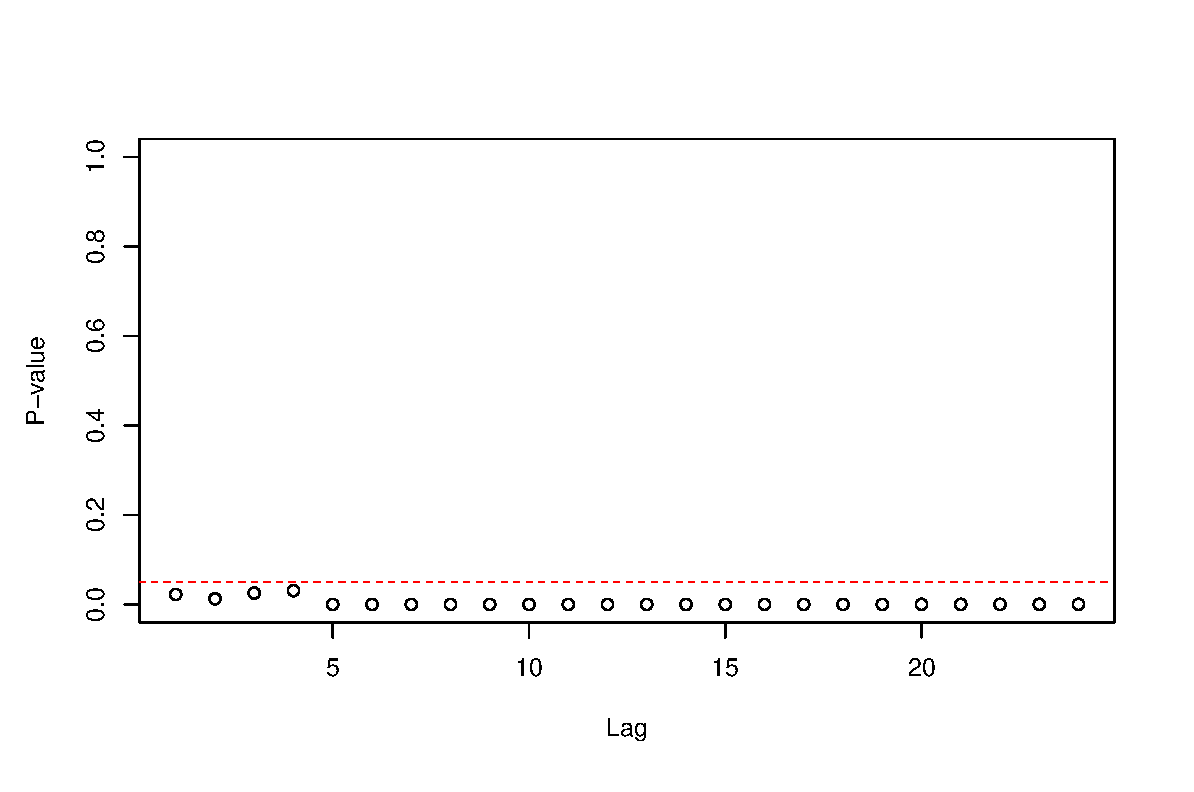
\includegraphics[width=0.5\linewidth]{pic/ast/mcr2}
	\caption{调整后序列的MA模型残差的McLeod.Li检验}
	\label{fig:mcr2}
\end{figure}
即现在的残差存在ARCH效应,需进一步建立异方差模型。利用rugarch包里的函数,建立MA(5)-GARCH(1,1)模型,残差分布为学生t分布。具体的参数估计结果如下(其中ma4不显著,置0):

\begin{framed}
	\begin{verbatim}
	 *---------------------------------*                         
	 *          GARCH Model Fit        *                           
	 *---------------------------------*
	 GARCH Model	: sGARCH(1,1)
	 Mean Model	: ARFIMA(0,0,5)
	 Distribution	: std 
	 ------------------------------------
	         Estimate  Std. Error  t value Pr(>|t|)
	 mu      2.198557    0.221154   9.9413 0.000000                                  
	 ma1     0.077369    0.067282   1.1499 0.250177
	 ma2     0.074749    0.058956   1.2679 0.204838
	 ma3     0.079972    0.050914   1.5707 0.116245
	 ma4     0.000000          NA       NA       NA
	 ma5     0.119163    0.050347   2.3668 0.017941
	 omega   5.250380    3.087206   1.7007 0.089001
	 alpha1  0.619542    0.378827   1.6354 0.101960
	 beta1   0.379458    0.151319   2.5077 0.012153
	 shape   2.897172    0.762001   3.8021 0.000143
	\end{verbatim}
\end{framed}
对模型进行诊断,见图\ref{fig:diagarch},
\begin{figure}[h!]
	\centering
	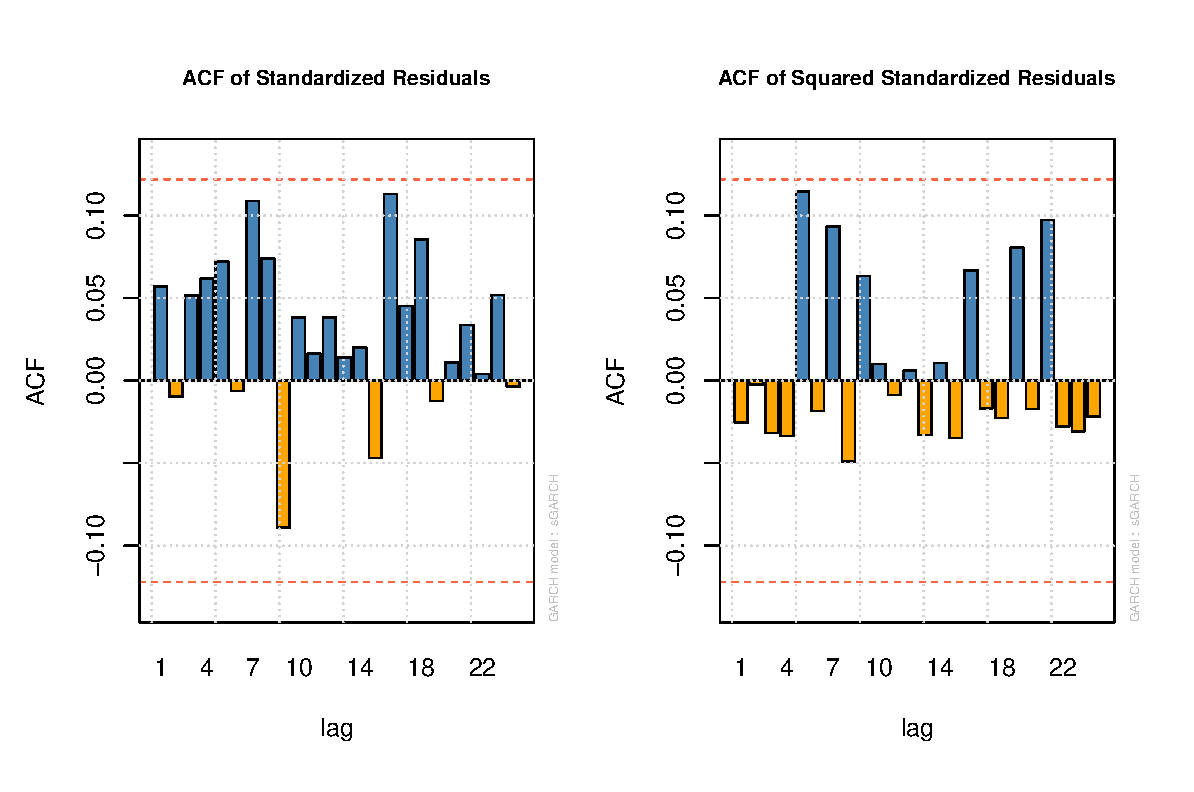
\includegraphics[width=0.7\linewidth]{pic/ast/diagarch}
	\caption{ARMA-GARCH模型诊断:左为标准化残差的ACF,右为标准化残差平方的ACF}
	\label{fig:diagarch}
\end{figure}
\begin{figure}[h!]
	\centering
	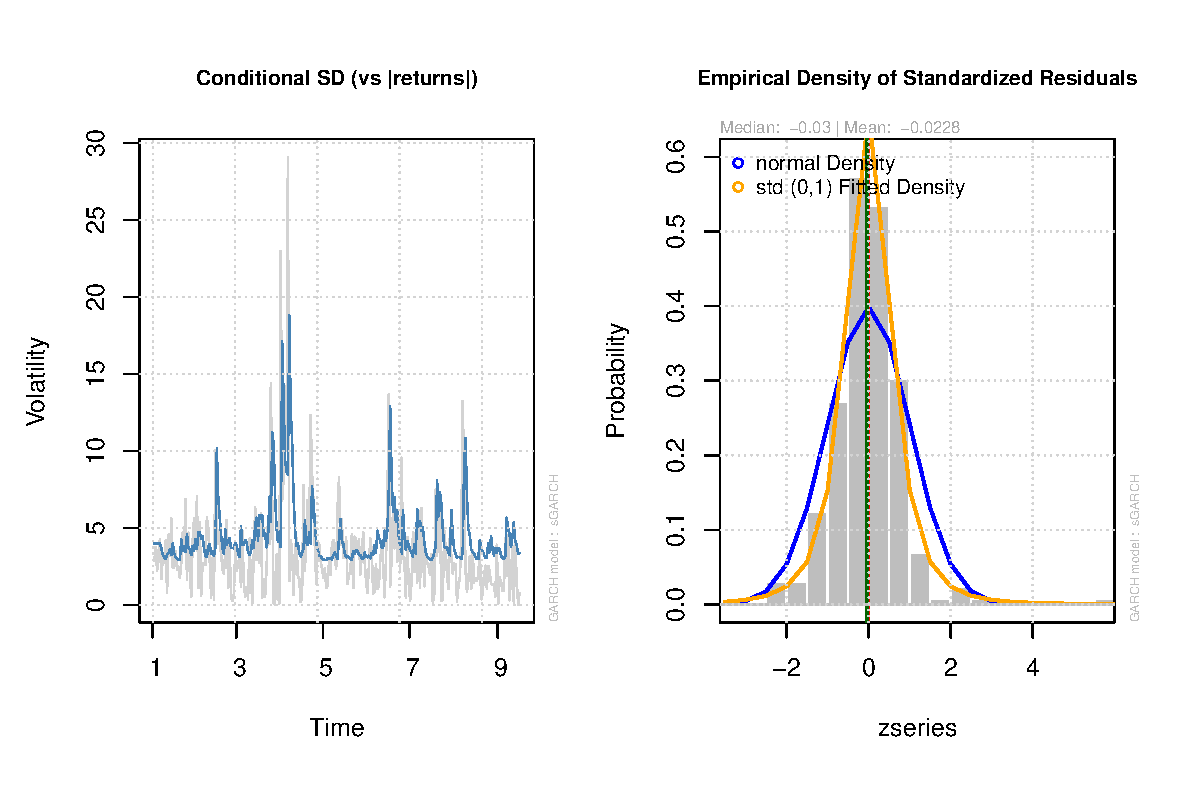
\includegraphics[width=0.6\linewidth]{pic/ast/diav}
	\caption{ARMA-GARCH模型诊断:左为模拟的残差波动与真实残差比较,右为模拟残差的std分布与标准正态分布比较}
	\label{fig:diav}
\end{figure}
可以直观看到其标准化残差不再具有一阶与二阶自相关性,这一点也可由GARCH模型结果中的"Ljung-Box Test on Standardized Residuals","Ljung-Box Test on Standardized Squared Residuals"和"ARCH LM Tests"的统计结果看到,具体可以运行附录里code即可重现,这里不再赘述。这说明现在的ARMA(0,5)-GARCH(1,1)模型是充分的。进一步见图\ref{fig:diav},可以看到对残差的t分布假设是合适的,其尾部比标准正态分布要厚,说明了FOF基金资产的对数增长率的波动,即风险,也存在尖峰厚尾的现象。
\begin{figure}[h!]
	\begin{minipage}[ht]{0.48\textwidth}
		\centering
		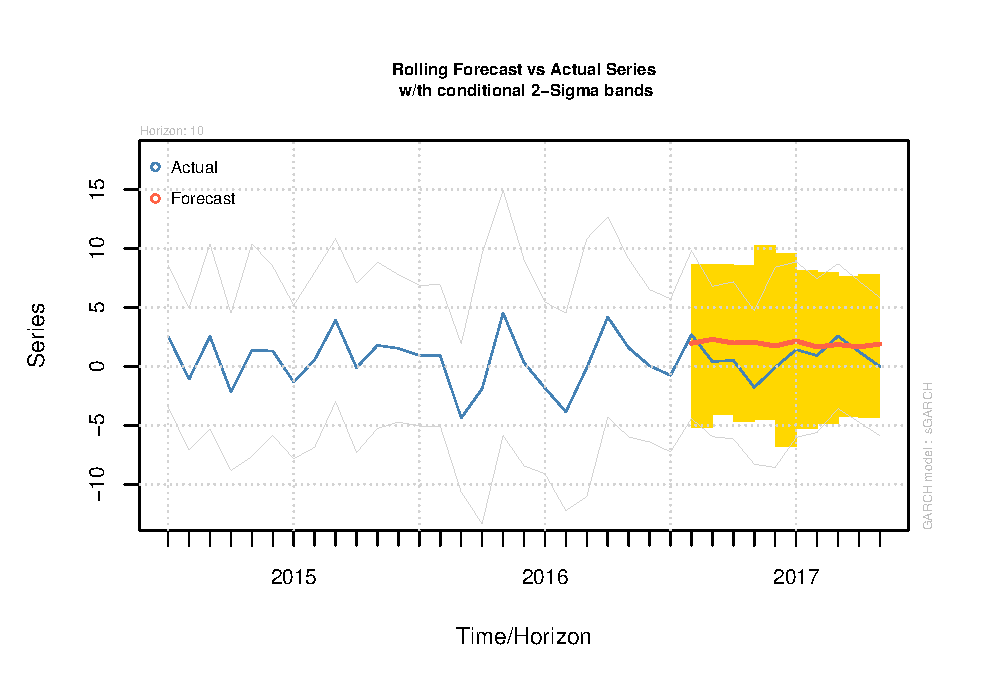
\includegraphics[width=\textwidth]{pic/ast/fastroll}
		\subcaption{}\label{fastroll}
	\end{minipage}%
	\hspace{0.04\textwidth}
	\begin{minipage}[ht]{0.48\textwidth}
		\centering
		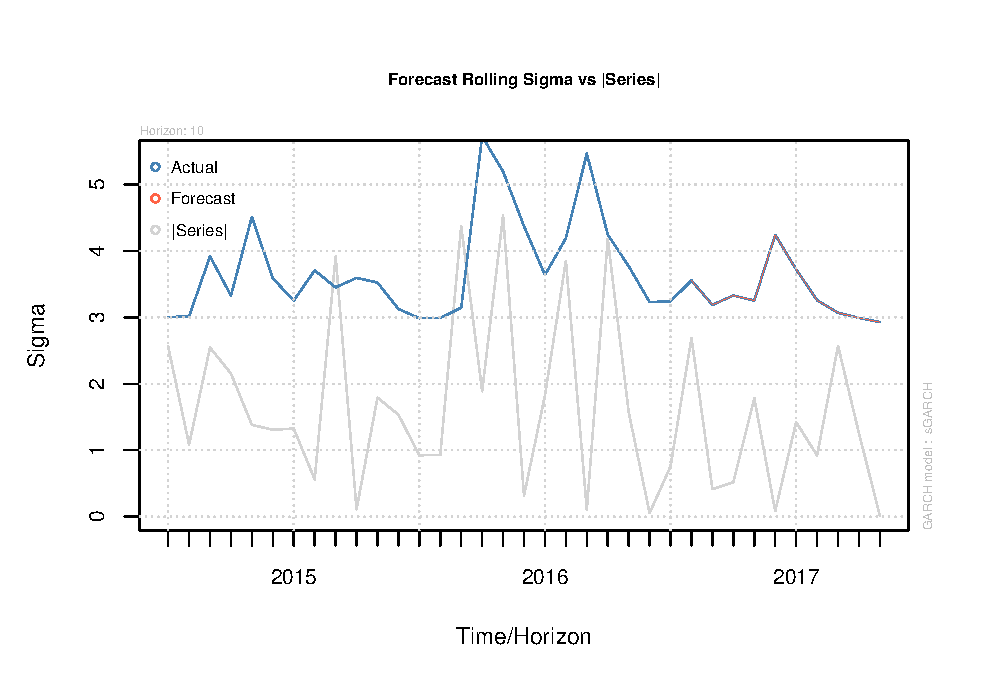
\includegraphics[width=\textwidth]{pic/ast/fastrollv}
		\subcaption{}\label{fastrollv}
	\end{minipage}
	\caption{利用ARMA(0,5)-GARCH(1,1)模型对调整后的FOF资产对数增长率及其波动方差进行滚动预测: (a):FOF资产对数增长率预测; (b):波动方差的滚动预测} \label{f}
\end{figure}
\par 现在可以利用上述模型进行预测分析如图\ref{f}所示,是序列值与序列波动方差的滚动预测,可以看到,对数增长率的预测相比与真实序列,较为平缓,但能有效反映出真实值的趋势,对预测未来值波动方向具有指导意义。对方差的预测,与真实值也符合的较好,能够反映出波动的大致方向。

% 图片使用了subfigure环境
% 表格都改为了 lstlisting环境
% 协整部分增加了解释
% 本节中所有的英文标点替换为中文标点
% 修正了其它的一些小错误
% ----------------------------------
% 修改了表格的排版
% ----------------------------------

\section{与退休养老资产的协整关系}
由于美国FOF基金的兴起, 主要源于养老金市场的发展. 美国雇员逐渐选择将养老金计划由DB(Defined Benefit) Plan转向DC(Defined Contribute) Plan, 增大了养老金投资着的投资需求. 而FOF基金作为一种收益稳定、风险二次分散的基金, 自然受到了这些被动投资者的青睐. 下面, 利用彭博数据库中FOF基金资产总量和养老金资产总量的季度数据, 对FOF基金市场与养老金市场进行协整分析. 在2007--2016十年中, 二者的绝对数量和增长率变化趋势如图~\ref{pic:3-0}~:



\begin{figure}[h!]
	\begin{minipage}[ht]{0.47\textwidth}
		\centering
		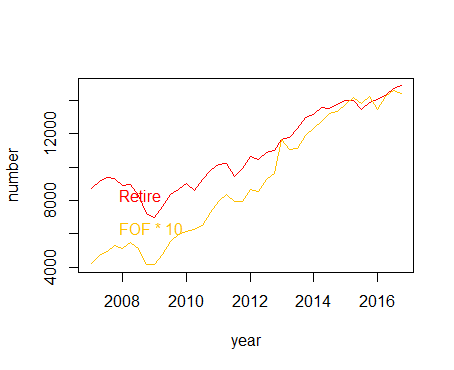
\includegraphics[width=1\textwidth]{pic/3-0-1.png}
		\subcaption{}\label{pic/3-0-1.png}
	\end{minipage}%
	\hspace{0.06\textwidth}
	\begin{minipage}[ht]{0.47\textwidth}
		\centering
		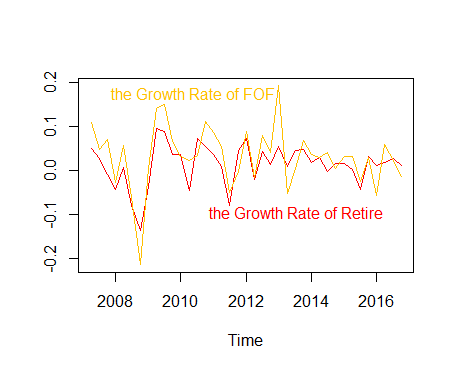
\includegraphics[width=1\textwidth]{pic/3-0-2.png}
		\subcaption{}\label{pic/3-0-2.png}
	\end{minipage}
	\caption{2007-2016年FOF基金和养老金发展情况季度数据:(a)1资产数量;(b)资产增长率} \label{pic:3-0}
\end{figure}





% 单位根检验部分
对$\{FOF\}$和$\{Retire\}$序列分别进行单位根检验.ADF检验和Phillips–Perron的结果接受了原假设(单位根过程), 并且Kwiatkowski–Phillips–Schmidt–Shin检验结果拒绝了原假设(平稳过程). 因此可以认为$\{FOF\}$和$\{Retire\}$是非平稳序列.
继续对它们的差分序列$\{\Delta FOF\}$和$\{\Delta Retire\}$进行单位根检验, 得到的结果表明它们是平稳序列. 所以, $\{FOF\}$和$\{Retire\}$分别是2个$I(1)$序列.下面对这两个序列进行协整估计.

% 单位根检验表格
\begin{framed}
\begin{verbatim}
 *---------------------------------*                         
 *          Unit Root Test         *                           
 *---------------------------------*
TEST Method      ADF       KPSS      PP  
FOF             2.53       1.07   -1.06
diff(FOF)      -3.40       0.11   40.00
Retire          1.64       1.01    0.23
diff(Retire)   -2.31       0.18    1.55
10pct          -1.61       0.35     *  
5pct           -1.95       0.46    0.26
1pct           -2.62       0.74     *  
\end{verbatim}
\end{framed}


% 协整部分
首先, 使用最小二乘法估计如下方程:
$$FOF_t = \alpha + \beta \cdot Retire_t + \mu_t$$
得到$\alpha$和$\beta$的估计量$\hat{\alpha}$和$\hat{\beta}$. 估计结果如下表所示:

% OLS回归结果表格
\begin{framed}
\begin{verbatim} 
Call:
lm(formula = fof ~ retire)

Residuals:
     Min       1Q   Median       3Q      Max 
-182.482  -26.622    1.348   38.330  145.811 

Coefficients:
              Estimate  Std Error t value Pr(>|t|)    
(Intercept) -7.552e+02  5.632e+01  -13.41 5.51e-16 ***
retire       1.524e-01  5.042e-03   30.22  < 2e-16 ***
---
Signif. codes:  0 '***' 0.001 '**' 0.01 '*' 0.05 '.' 0.1 ' ' 1

Residual standard error: 74.18 on 38 degrees of freedom
Multiple R-squared:  0.9601,    Adjusted R-squared:  0.959 
F-statistic: 913.5 on 1 and 38 DF,  p-value: < 2.2e-16
\end{verbatim}
\end{framed}



对残差估计序列$\{\hat{\mu}\}$进行单位根检验, $\{\hat{\mu}\}$在ADF检验和PP检验中拒绝了存在单位根的原假设, 在KPSS检验中接受了序列平稳的原假设.因此可以认为$\{FOF\}$和$\{Retire\}$两个$I(1)$过程得到了平稳的$I(0)$
过程. 即两个序列之间存在着长期的均衡关系(协整关系). 协整向量为$(1, -0.15)$.

% 残差具有平稳性
\begin{framed}
\begin{verbatim}
 *---------------------------------------------------------*
 *                      Unit Root Test                     *
 *---------------------------------------------------------*    
TESTs             ADF-Test       KPSS-Test           PP-Test
Statistics   -3.18 (<1pct)   0.27 (<10pct)   -10.04 (<Z-tau)
\end{verbatim}
\end{framed}

% Error Correction Model
记$y_t = FOF_t$, $x_t = Retire_t$, 建立误差修正模型. 由于使用的是季度数据, 所以加入$\Delta y_t$的1--4阶滞后项.误差修正方程如下:
$$
\Delta y_t = \alpha_1 \cdot \Delta y_{t-1} + \alpha_2  \cdot \Delta  y_{t-2} + \alpha_3 \cdot \Delta  y_{t-3} + \alpha_4 \cdot \Delta  y_{t-4} + \beta_0 \cdot \Delta  x_t+\beta_1 \cdot \Delta  x_{t-1} + \gamma \cdot ( y_{t-1}-kx_{t-1}) + \epsilon_t
$$


估计结果如下表所示:

% 误差修正模型的估计结果
\begin{framed}
\begin{verbatim}
 *---------------------------------------------------------*
 *                 Error Correction Model                  *
 *---------------------------------------------------------* 
Call:
dynlm(formula = y ~ L(y, 1) + L(y, 2) + L(y, 3) + L(y, 4) + L(x, 
    1) + L(x, 0) + L(r, 1), data = ecmdat1)

Residuals:
    Min      1Q  Median      3Q     Max 
-87.387 -20.436   1.006  16.815 142.580 

Coefficients:
            Estimate Std. Error t value Pr(>|t|)    
(Intercept) 22.13335   11.14436   1.986   0.0573 .  
L(y, 1)     -0.46108    0.19994  -2.306   0.0290 *  
L(y, 2)     -0.01601    0.12908  -0.124   0.9022    
L(y, 3)     -0.03563    0.12999  -0.274   0.7861    
L(y, 4)     -0.02875    0.13862  -0.207   0.8373    
L(x, 1)      0.05842    0.02549   2.292   0.0300 *  
L(x, 0)      0.09517    0.01852   5.138  2.1e-05 ***
L(r, 1)     -0.38373    0.16855  -2.277   0.0309 *  
---
Signif. codes:  0 '***' 0.001 '**' 0.01 '*' 0.05 '.' 0.1 ' ' 1

Residual standard error: 40.94 on 27 degrees of freedom
Multiple R-squared:  0.5683,    Adjusted R-squared:  0.4564 
F-statistic: 5.078 on 7 and 27 DF,  p-value: 9e-04
\end{verbatim}
\end{framed}


协整方程的估计结果为
$$\Delta y_t =22.13  -0.46 \cdot \Delta y_{t-1} -0.01 \cdot \Delta  y_{t-2}   -0.04 \cdot \Delta  y_{t-3}  -0.03 \cdot \Delta  y_{t-4} + 0.10 \cdot \Delta  x_t+ 0.06 \cdot \Delta  x_{t-1} -0.38 \cdot ( y_{t-1}-0.15x_{t-1}) + \epsilon_t$$
$\Delta y$的滞后项中,只有一期滞后项是显著的;误差修正项的系数为-0.38,在10\%的程度显著,符合反向修正机制. 协整向量为$(1, -0.15)$.
ECM模型说明FOF基金市场和养老金市场存在长期的稳定关系(图~\ref{fg:coin-result}~).从资产数量的角度上,养老金市场的发展推动了FOF基金市场的发展;长期均衡中,FOF基金的资产总量维持在养老金市场资产总量的15\%.而上一期的不均衡误差对当期以38\%的比率进行修正.

\begin{figure}[h!]
  \centering
  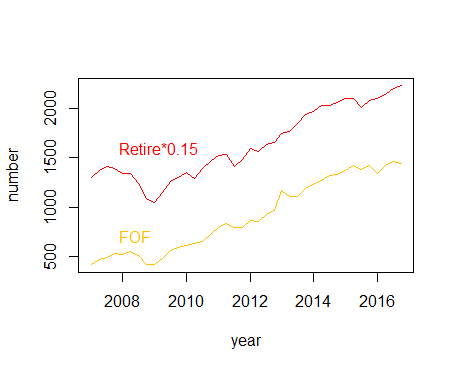
\includegraphics[width=0.6\textwidth]{pic/coin-result.png}
  \caption{长期均衡关系}\label{fg:coin-result}
\end{figure}

美国养老金体系包括政府主办的退休金保险、雇主资助的私营养老金、个人储蓄多个层次.从DB Plan(确定收益计划)到DC Plan(确定退休金计划)的演变,使得雇员更多地考虑到投资工具的收益的稳定性.
而共同基金,特别是FOF是养老金的理想投资工具.和其它投资工具相比,FOF基金具有一些天然的投资优势:(1)低风险性,基金本身通过组合的方式,对股票和证券进行了资产分散;而FOF基金则通过投资不同类型基金,进行双重的风险分散,从而能够获得更加稳定的收益;(2)降低了多样化投资门槛,投资者不再需要繁复地挑选基金,可以通过只投资一个产品来获得相似的投资效果.

借鉴美国养老金与FOF市场的关联关系的实证经验,可以对中国市场得到启示.2016年末,中国社保基金资产总额达到20,423.28亿元.而中国社会提前进入老龄化社会,使得养老保险制度面临更大的挑战.
目前,中国资本市场还不成熟, 特别是股票市场波动较大,存在着资产质量报告及信息不对称、庄家操纵股价等一系列的问题 ,而且缺乏有效的避险工具.在这样的情况下,选择稳定收益的投资工具十分重要.
此外,由美国市场的经验,养老金市场的发展也在推动了FOF基金的发展.养老金成熟的投资于FOF基金,也会促进FOF基金的发展,进而推动共同基金市场的发展.


\section{结论}
    \begin{enumerate}
        \item 在过去的20年中, FOF资产总量的增长率满足ARMA(0,5)-GARCH(1,1)模型.
        \item FOF基金市场和养老金市场之前存在协整关系. FOF资产总量维持在养老金市场总量的15\%水平, 可以实现长期稳定关系.
    \end{enumerate}

\textcolor{red}{修改:把结论第一点再说具体一些,现在字数有点少,by王喆}
\clearpage



\clearpage



\appendix
\section{数据}
\subsection{美国基金中基金市场的规模}
\begin{center}
\begin{longtable}{rr|rr|rr}
\caption{1995年1月至2017年5月美国基金中基金市场的规模\label{tab:fof}}\\
\hline\hline
    \multicolumn{1}{c}{\multirow{2}[0]{*}{\textbf{时间}}} & \multicolumn{1}{c|}{\textbf{资产}} & \multicolumn{1}{c}{\multirow{2}[0]{*}{\textbf{时间}}} & \multicolumn{1}{c|}{\textbf{资产}} & \multicolumn{1}{c}{\multirow{2}[0]{*}{\textbf{时间}}} & \multicolumn{1}{c}{\textbf{资产}} \\
          & \multicolumn{1}{c|}{\textbf{(百万美元)}} &       & \multicolumn{1}{c|}{\textbf{(百万美元)}} &       & \multicolumn{1}{c}{\textbf{(百万美元)}} \\
\hline
\endfirsthead
\multicolumn{6}{c}%
{\tablename\ \thetable\ -- \textit{接上页}} \\
\hline
    \multicolumn{1}{c}{\multirow{2}[0]{*}{\textbf{时间}}} & \multicolumn{1}{c|}{\textbf{资产}} & \multicolumn{1}{c}{\multirow{2}[0]{*}{\textbf{时间}}} & \multicolumn{1}{c|}{\textbf{资产}} & \multicolumn{1}{c}{\multirow{2}[0]{*}{\textbf{时间}}} & \multicolumn{1}{c}{\textbf{资产}} \\
          & \multicolumn{1}{c|}{\textbf{(百万美元)}} &       & \multicolumn{1}{c|}{\textbf{(百万美元)}} &       & \multicolumn{1}{c}{\textbf{(百万美元)}} \\
\hline
\endhead
\hline \multicolumn{6}{r}{\textit{接下页}} \\
\endfoot
\hline\hline \multicolumn{6}{r}{\textit{数据来源: bloomberg}}
\endlastfoot
    1995/01 & 3891.54 & 1995/02 & 4004.15 & 1995/03 & 4157.77 \\
    1995/04 & 4251.60 & 1995/05 & 4402.44 & 1995/06 & 4593.91 \\
    1995/07 & 4672.64 & 1995/08 & 4823.46 & 1995/09 & 4958.94 \\
    1995/10 & 5171.76 & 1995/11 & 5213.18 & 1995/12 & 5457.18 \\
    1996/01 & 5633.96 & 1996/02 & 5960.12 & 1996/03 & 6106.85 \\
    1996/04 & 6257.97 & 1996/05 & 6480.18 & 1996/06 & 6632.46 \\
    1996/07 & 6800.38 & 1996/08 & 6682.34 & 1996/09 & 6865.76 \\
    1996/10 & 7197.85 & 1996/11 & 7459.89 & 1996/12 & 7989.89 \\
    1997/01 & 8123.58 & 1997/02 & 8514.52 & 1997/03 & 8699.14 \\
    1997/04 & 8649.68 & 1997/05 & 9020.01 & 1997/06 & 9543.86 \\
    1997/07 & 9925.52 & 1997/08 & 10648.88 & 1997/09 & 10530.58 \\
    1997/10 & 11112.78 & 1997/11 & 11044.41 & 1997/12 & 11352.39 \\
    1998/01 & 11655.81 & 1998/02 & 11963.02 & 1998/03 & 12664.41 \\
    1998/04 & 13294.74 & 1998/05 & 13683.06 & 1998/06 & 13746.65 \\
    1998/07 & 14179.25 & 1998/08 & 14128.49 & 1998/09 & 12777.88 \\
    1998/10 & 13300.41 & 1998/11 & 13964.41 & 1998/12 & 14532.98 \\
    1999/01 & 15022.44 & 1999/02 & 15376.77 & 1999/03 & 15066.40 \\
    1999/04 & 15608.80 & 1999/05 & 16495.46 & 1999/06 & 16311.59 \\
    1999/07 & 16957.58 & 1999/08 & 16863.42 & 1999/09 & 16819.18 \\
    1999/10 & 16701.55 & 1999/11 & 17332.58 & 1999/12 & 17721.58 \\
    2000/01 & 18214.94 & 2000/02 & 17662.49 & 2000/03 & 17873.37 \\
    2000/04 & 18751.00 & 2000/05 & 18496.00 & 2000/06 & 18396.02 \\
    2000/07 & 18612.33 & 2000/08 & 18678.35 & 2000/09 & 19502.83 \\
    2000/10 & 19172.91 & 2000/11 & 19151.47 & 2000/12 & 18528.61 \\
    2001/01 & 19749.24 & 2001/02 & 20338.12 & 2001/03 & 19507.07 \\
    2001/04 & 18978.33 & 2001/05 & 20144.45 & 2001/06 & 20245.34 \\
    2001/07 & 19905.22 & 2001/08 & 20014.13 & 2001/09 & 19558.66 \\
    2001/10 & 18492.07 & 2001/11 & 19243.60 & 2001/12 & 22221.82 \\
    2002/01 & 20769.81 & 2002/02 & 20746.55 & 2002/03 & 20755.45 \\
    2002/04 & 21449.55 & 2002/05 & 21321.43 & 2002/06 & 21301.30 \\
    2002/07 & 45669.03 & 2002/08 & 42665.45 & 2002/09 & 46329.04 \\
    2002/10 & 51587.31 & 2002/11 & 57018.59 & 2002/12 & 76280.67 \\
    2003/01 & 75090.64 & 2003/02 & 71979.21 & 2003/03 & 74544.03 \\
    2003/04 & 75032.41 & 2003/05 & 77723.33 & 2003/06 & 81166.19 \\
    2003/07 & 82694.96 & 2003/08 & 84115.64 & 2003/09 & 84286.23 \\
    2003/10 & 83845.05 & 2003/11 & 90622.28 & 2003/12 & 92661.04 \\
    2004/01 & 97158.40 & 2004/02 & 104011.11 & 2004/03 & 108635.58 \\
    2004/04 & 122895.62 & 2004/05 & 133983.55 & 2004/06 & 143331.71 \\
    2004/07 & 148663.38 & 2004/08 & 150728.16 & 2004/09 & 156230.53 \\
    2004/10 & 162639.36 & 2004/11 & 167402.90 & 2004/12 & 171383.94 \\
    2005/01 & 174442.90 & 2005/02 & 178663.61 & 2005/03 & 180644.12 \\
    2005/04 & 183032.82 & 2005/05 & 188376.19 & 2005/06 & 192123.44 \\
    2005/07 & 199859.87 & 2005/08 & 208480.39 & 2005/09 & 215081.04 \\
    2005/10 & 220273.78 & 2005/11 & 234997.47 & 2005/12 & 255266.06 \\
    2006/01 & 265454.38 & 2006/02 & 280590.70 & 2006/03 & 289272.48 \\
    2006/04 & 299346.94 & 2006/05 & 312759.22 & 2006/06 & 317089.00 \\
    2006/07 & 323568.98 & 2006/08 & 330218.35 & 2006/09 & 345766.22 \\
    2006/10 & 349620.43 & 2006/11 & 365517.94 & 2006/12 & 381525.97 \\
    2007/01 & 395654.18 & 2007/02 & 413001.92 & 2007/03 & 421266.16 \\
    2007/04 & 435453.75 & 2007/05 & 456568.17 & 2007/06 & 469966.94 \\
    2007/07 & 477194.84 & 2007/08 & 480902.06 & 2007/09 & 493065.61 \\
    2007/10 & 514898.91 & 2007/11 & 533376.36 & 2007/12 & 529529.30 \\
    2008/01 & 534289.55 & 2008/02 & 520191.05 & 2008/03 & 514646.96 \\
    2008/04 & 508470.37 & 2008/05 & 523082.91 & 2008/06 & 544725.97 \\
    2008/07 & 529515.72 & 2008/08 & 526861.80 & 2008/09 & 512458.99 \\
    2008/10 & 479500.51 & 2008/11 & 418175.57 & 2008/12 & 413135.16 \\
    2009/01 & 425735.13 & 2009/02 & 399602.82 & 2009/03 & 414628.09 \\
    2009/04 & 441387.68 & 2009/05 & 454104.29 & 2009/06 & 478017.71 \\
    2009/07 & 489189.85 & 2009/08 & 538315.04 & 2009/09 & 556143.45 \\
    2009/10 & 571690.68 & 2009/11 & 569009.49 & 2009/12 & 594713.21 \\
    2010/01 & 603296.68 & 2010/02 & 604997.72 & 2010/03 & 613747.34 \\
    2010/04 & 643478.26 & 2010/05 & 657422.41 & 2010/06 & 627196.83 \\
    2010/07 & 618079.94 & 2010/08 & 656942.36 & 2010/09 & 649672.88 \\
    2010/10 & 691727.30 & 2010/11 & 717014.97 & 2010/12 & 725812.87 \\
    2011/01 & 751328.49 & 2011/02 & 772202.43 & 2011/03 & 791899.00 \\
    2011/04 & 807483.61 & 2011/05 & 834704.22 & 2011/06 & 835778.39 \\
    2011/07 & 830000.85 & 2011/08 & 769909.22 & 2011/09 & 794900.02 \\
    2011/10 & 748423.04 & 2011/11 & 795681.22 & 2011/12 & 793597.63 \\
    2012/01 & 796472.81 & 2012/02 & 836033.37 & 2012/03 & 867648.22 \\
    2012/04 & 884599.71 & 2012/05 & 893903.72 & 2012/06 & 853352.89 \\
    2012/07 & 880810.17 & 2012/08 & 899012.82 & 2012/09 & 923559.21 \\
    2012/10 & 948199.53 & 2012/11 & 950534.35 & 2012/12 & 962415.61 \\
    2013/01 & 979779.23 & 2013/02 & 1022456.88 & 2013/03 & 1167128.29 \\
    2013/04 & 1073323.00 & 2013/05 & 1097449.88 & 2013/06 & 1107170.36 \\
    2013/07 & 1089874.24 & 2013/08 & 1124873.00 & 2013/09 & 1113023.58 \\
    2013/10 & 1153404.90 & 2013/11 & 1170515.85 & 2013/12 & 1191252.26 \\
    2014/01 & 1210088.64 & 2014/02 & 1187520.60 & 2014/03 & 1234096.87 \\
    2014/04 & 1238799.16 & 2014/05 & 1247947.58 & 2014/06 & 1271898.35 \\
    2014/07 & 1304877.84 & 2014/08 & 1290804.96 & 2014/09 & 1324078.57 \\
    2014/10 & 1295844.43 & 2014/11 & 1313867.10 & 2014/12 & 1331161.52 \\
    2015/01 & 1313628.87 & 2015/02 & 1321029.56 & 2015/03 & 1373800.97 \\
    2015/04 & 1372278.97 & 2015/05 & 1397090.52 & 2015/06 & 1418694.42 \\
    2015/07 & 1431861.66 & 2015/08 & 1445206.70 & 2015/09 & 1383349.54 \\
    2015/10 & 1357479.17 & 2015/11 & 1420458.98 & 2015/12 & 1424948.06 \\
    2016/01 & 1399192.81 & 2016/02 & 1346345.30 & 2016/03 & 1344888.45 \\
    2016/04 & 1402333.30 & 2016/05 & 1424562.38 & 2016/06 & 1425313.57 \\
    2016/07 & 1414559.58 & 2016/08 & 1453163.33 & 2016/09 & 1459183.73 \\
    2016/10 & 1466733.52 & 2016/11 & 1440816.65 & 2016/12 & 1439637.04 \\
    2017/01 & 1460271.42 & 2017/02 & 1473791.88 & 2017/03 & 1512170.81 \\
    2017/04 & 1531286.24 & 2017/05 & 1531106.44 &       &  \\
\end{longtable}
\end{center}

\subsection{美国退休养老资产规模}
\begin{footnotesize}
\begin{center}
\begin{longtable}{rrrrrrrr}
  \caption{2007年1季度至2016年4季度美国退休养老资产规模~~(单位:十亿美元)\label{tab:retire}}\\
\hline\hline
    \multirow{2}[0]{*}{\textbf{Time}} & \multirow{2}[0]{*}{\textbf{IRAs}} & \textbf{\tiny DC} & \textbf{\tiny Private-Sector} & \textbf{\tiny Government} & \textbf{\tiny Federal} & \multirow{2}[0]{*}{\textbf{Annuities}} & \multirow{2}[0]{*}{\textbf{Total}} \\
          &       & \textbf{\tiny Plans} & \textbf{\tiny DB Plans} & \textbf{\tiny DB Plans} & \textbf{\tiny DB Plans} &       &  \\
\hline
\endfirsthead
\multicolumn{8}{c}%
{\tablename\ \thetable\ -- \textit{接上页}} \\
\hline
    \multirow{2}[0]{*}{\textbf{Time}} & \multirow{2}[0]{*}{\textbf{IRAs}} & \textbf{\tiny DC} & \textbf{\tiny Private-Sector} & \textbf{\tiny Government} & \textbf{\tiny Federal} & \multirow{2}[0]{*}{\textbf{Annuities}} & \multirow{2}[0]{*}{\textbf{Total}} \\
          &       & \textbf{\tiny Plans} & \textbf{\tiny DB Plans} & \textbf{\tiny DB Plans} & \textbf{\tiny DB Plans} &       &  \\
\hline
\endhead
\hline \multicolumn{8}{r}{\textit{接下页}} \\
\endfoot
\hline\hline \multicolumn{8}{r}{\textit{数据来源: Investment Company Institute (ICI)}}
\endlastfoot
    2007:Q1 & 4340  & 4360  & 2520  & 3161  & 930   & 1431  & 16742  \\
    2007:Q2 & 4605  & 4535  & 2675  & 3308  & 920   & 1488  & 17531  \\
    2007:Q3 & 4775  & 4614  & 2685  & 3352  & 936   & 1516  & 17878  \\
    2007:Q4 & 4748  & 4555  & 2646  & 3296  & 978   & 1507  & 17730  \\
    2008:Q1 & 4555  & 4356  & 2515  & 3120  & 961   & 1442  & 16948  \\
    2008:Q2 & 4580  & 4396  & 2495  & 3132  & 967   & 1432  & 17002  \\
    2008:Q3 & 4225  & 4069  & 2340  & 2944  & 984   & 1369  & 15931  \\
    2008:Q4 & 3681  & 3547  & 1979  & 2466  & 1033  & 1239  & 13946  \\
    2009:Q1 & 3536  & 3429  & 1840  & 2288  & 1009  & 1193  & 13296  \\
    2009:Q2 & 3925  & 3736  & 1990  & 2407  & 1015  & 1275  & 14347  \\
    2009:Q3 & 4325  & 4053  & 2155  & 2619  & 1032  & 1363  & 15546  \\
    2009:Q4 & 4488  & 4200  & 2228  & 2728  & 1095  & 1397  & 16137  \\
    2010:Q1 & 4644  & 4373  & 2315  & 2833  & 1079  & 1439  & 16683  \\
    2010:Q2 & 4405  & 4204  & 2210  & 2623  & 1081  & 1392  & 15915  \\
    2010:Q3 & 4757  & 4500  & 2345  & 2762  & 1099  & 1482  & 16944  \\
    2010:Q4 & 5029  & 4758  & 2481  & 2954  & 1161  & 1557  & 17941  \\
    2011:Q1 & 5255  & 4903  & 2545  & 3049  & 1147  & 1606  & 18504  \\
    2011:Q2 & 5315  & 4927  & 2535  & 3004  & 1155  & 1614  & 18550  \\
    2011:Q3 & 4910  & 4538  & 2440  & 2673  & 1165  & 1512  & 17238  \\
    2011:Q4 & 5153  & 4738  & 2525  & 2838  & 1230  & 1574  & 18057  \\
    2012:Q1 & 5550  & 5089  & 2685  & 3048  & 1214  & 1672  & 19259  \\
    2012:Q2 & 5450  & 4981  & 2640  & 2951  & 1220  & 1635  & 18878  \\
    2012:Q3 & 5700  & 5186  & 2723  & 3025  & 1239  & 1688  & 19562  \\
    2012:Q4 & 5785  & 5242  & 2709  & 2998  & 1270  & 1705  & 19709  \\
    2013:Q1 & 6123  & 5535  & 2790  & 3190  & 1282  & 1756  & 20675  \\
    2013:Q2 & 6189  & 5587  & 2775  & 3240  & 1287  & 1758  & 20836  \\
    2013:Q3 & 6487  & 5848  & 2808  & 3349  & 1301  & 1816  & 21609  \\
    2013:Q4 & 6819  & 6132  & 2892  & 3549  & 1370  & 1886  & 22648  \\
    2014:Q1 & 6961  & 6212  & 2910  & 3559  & 1357  & 1899  & 22898  \\
    2014:Q2 & 7215  & 6352  & 2968  & 3641  & 1360  & 1939  & 23475  \\
    2014:Q3 & 7182  & 6367  & 2949  & 3630  & 1378  & 1925  & 23431  \\
    2014:Q4 & 7292  & 6480  & 3003  & 3730  & 1438  & 1954  & 23896  \\
    2015:Q1 & 7445  & 6547  & 3003  & 3756  & 1417  & 1976  & 24145  \\
    2015:Q2 & 7504  & 6522  & 2972  & 3772  & 1419  & 1979  & 24168  \\
    2015:Q3 & 7133  & 6298  & 2828  & 3551  & 1439  & 1910  & 23160  \\
    2015:Q4 & 7329  & 6537  & 2870  & 3664  & 1512  & 1954  & 23866  \\
    2016:Q1 & 7400  & 6639  & 2863  & 3665  & 1497  & 1976  & 24041  \\
    2016:Q2 & 7527  & 6775  & 2876  & 3714  & 1497  & 2004  & 24392  \\
    2016:Q3 & 7767  & 6938  & 2916  & 3813  & 1515  & 2045  & 24992  \\
    2016:Q4 & 7850  & 7028  & 2946  & 3861  & 1595  & 2049  & 25330  \\
\end{longtable}
\end{center}
\end{footnotesize} 
\section{代码}
\textcolor{red}{请二位模仿我下面写的这样,补充上各自负责的那一部分的代码,注意写清楚subsection,做好命名。如果自己一个人的代码太多,放在一起太混乱,可以写多个subsection,by王喆\& RQJ}

\textcolor{red}{正文部分如果需要展示R的输出,也可以用下面的这个lstlisting环境,可能会比table环境更适合一些,by王喆\& RQJ}
\subsection{xxxxxxx}
\begin{lstlisting}[language=R,frame=single]
rm(list=ls())

library(readxl)
library(TSA)
library(forecast)

data <- read_excel("API.xlsx", sheet = "R", col_types = c("skip", "numeric", "numeric"))

ast = data[1] # ast represents asset
ast = ts(ast, frequency = 12,start = c(1995,1)) # total net assets

GR_ast = diff(log(ast)) # growth ratio of total net asset
GR_ast = ts(GR_ast * 100, frequency = 12,start = c(1995,2), names = 'GR_ast')

par(mfrow = c(2,1))
plot(ast)
plot(GR_ast)

adf.test(ast)
adf.test(GR_ast)
\end{lstlisting}

\end{document}
